\section{AVNA1 Vector Voltmeter  (VVM)}
\label{sect:VVM}
The AVNA allows measurement of the gain of a device, using an internal signal generator.  This is presented in terms of dB change in amplitude and shift in phase angle between the input and output.  This most useful for characterizing a device, such as a filter.  To do this, we have indeed built a voltmeter to measure the device output.  Sometimes we would just like to see the voltage displayed directly.  This lets us probe circuits for troubleshooting  and design work.   That is what the VVM does for us.

Phase information is important for some network diagnosis.  The VVM is intended to be used with the internal signal generator when phase is to be read.

\subsection{Description}
\label{subsect:VVMDescr}
The Vector Voltmeter measures the input rms voltage at any frequency up to about 40 kHz.  The frequency of the VVM is determined by the frequency of Signal Generator 1 (SG\#1).  Additionally, the phase difference between SG\#1 and the input signal is displayed.  By using the SG\#1 output to drive the test circuit, this phase is constant and can be a useful diagnostic tool.   If an external generator is used, the measured phase difference will change at a rate determined by the frequency difference between the SG\#1 set frequency and the external generator.    This, too, can be a useful measurement.  

The bandwidth of the measurement is only a few Hz making the measurement very sensitive, \textit{i.e.}, low noise.  The VVM operates down into the microVolt  region.

\subsection{Instructions}
\label{subsect:VVMInstr}
\textbf{Using the VVM - }Operation starts  by setting the frequency of SG\#1 to that appropriate for the measurement.  The generator does not need to be enabled ("On") if the signal source for the measurement is generated externally.  If the internal SG\#1 is used as the signal source, it should be enabled and the amplitude set.   Only the frequency setting will affect the VVM measurement.  The steps for controlling the signal generator are listed in the Section 6, below.

If it is possible to do so, the internal SG\#1 should be used as the signal source, and this is a requirement if phase needs to be constant and representative of the circuit.

Again starting from the main home screen Figure \ref{AVNA_000-label}, we tap the "\textsf{Vector VMeter}" button on the bottom row.  This brings up the single screen used by the VVM.  It will be displaying amplitude in \textsf{Volts RMS}  and phase in degrees, with both shown in bold numbers.  With no input, these parameters should be low in value, with the exact voltage depending on frequency.  The example of Figure  \ref{AVNA_015-label} is running at 996 Hz,with the input shorted to ground, and shows 9 microVolts RMS.
%
\begin{figure}[H]
\begin{center}
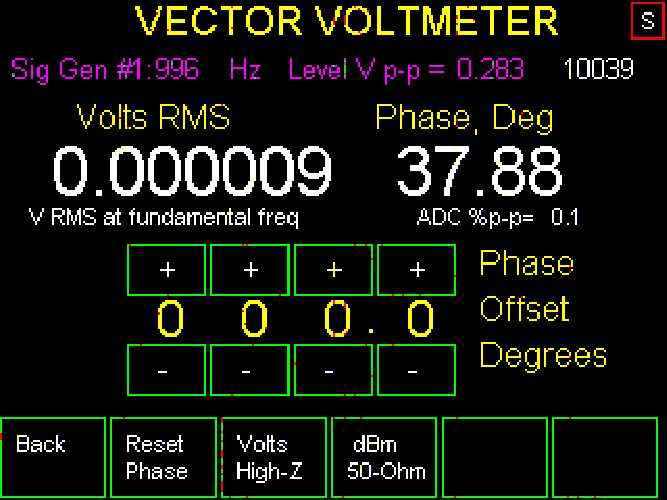
\includegraphics[scale=0.75]{./images/AVNA_015.pdf}
\caption{Vector Voltmeter, ready to measure but with no input.}
\label{AVNA_015-label}
\end{center}
\end{figure}
%
On the second from top text row is a notation in red, "\textsf{SigGen \#1 996 Hz}" that shows us the SG\#1 frequency without going back to the Signal Generator screens.  If SG\#1 is on (enabled), the frequency is shown in white; otherwise it is shown in pink/red.

We can now measure a voltage at the chosen frequency by connecting an input to the T input terminals.  The voltage amplitude shown is valid regardless of whether the 50-Ohm switch is on or off.  The load of the 50-Ohms may cut the amplitude, but the voltage across the resistor is accurate.  Figure  \ref{AVNA_016-label} shows the resulting screen.
%
\begin{figure}[H]
\begin{center}
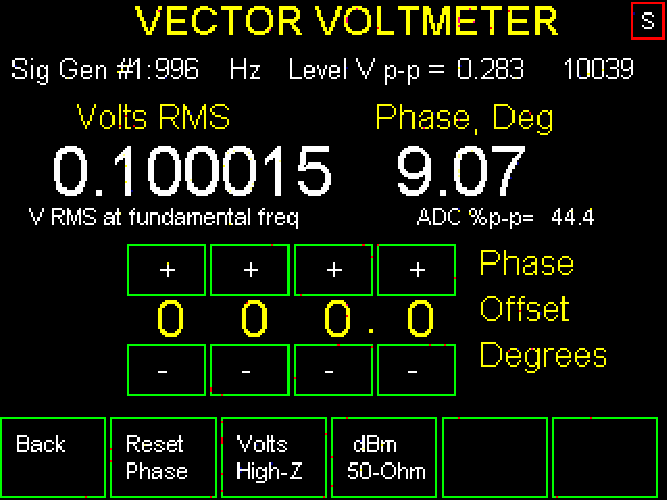
\includegraphics[scale=0.75]{./images/AVNA_016.pdf}
\caption{Vector Voltmeter with Sig Gen \#1 on and connected across to the VVM input.}
\label{AVNA_016-label}
\end{center}
\end{figure}
%
We can see that the input voltage is 0.100 Volts RMS..  From the second line, we see that the frequency of operation is 996 Hz, but it shows the level as 0.283 Vp-p.  These, of course, represent the same level  as the peak voltage is $\sqrt{2} = 1.414$ times the RMS voltage and peak-to-peak is twice the peak value.   This mixed units for the voltage is a complicated issue, probably makes sense but unfortunately causes more mental exercise than one might want, at times.

 Getting back to the VVM, you can see how close you are to overload by the little "\textsf{ADC \%p-p=xx.x}" on the screen.  This is the per cent of full ADC range for  the input.  If the level gets to 100\%, the voltage display turns red.  At that point the measurements are invalid.

Below the voltage and phase display is a "\textsf{Phase Offset}" input.  This can be set to values from -180 to +180 degrees.  This is a convenience that allows relative phase measurements to be made directly on the display.  This does not restrict the range of phase measurements, and they will always display between -180 and +180 degrees.

\textbf{Input Impedance - }One more convenience is the two buttons that select "\textsf{Volts High-Z}" or "\textsf{dBm-50 Ohms}".  For the  dBm readout to be correct, it is necessary to 50-Ohm terminate the input; this is easily done with the "50-Ohm" slide switch.  The resulting display  in Figure  \ref{AVNA_018-label} is shown below.  Note that along with switching the amplitude units,  a phase offset that has been used to bring the phase display to 0.00 (almost).

When the 50-Ohm switch is not closed, the input impedance is one Megohm in parallel with about 25 pF.  This is the input impedance of many oscilloscopes, meaning that  various x10 and x100 probes can be used with the VVM (as well as with the Spectrum Analyzer) to increase measurement voltage range and to add isolation from a circuit being measured. \textbf{A Warning - }An oscilloscope comes with input protection circuits that we do not have in the AVNA1. That means it is easy to damage the AVNA1. Keep the input at the box to a Volt or so and everything will be OK. Big voltages can cause damage. 
%
\begin{figure}[H]
\begin{center}
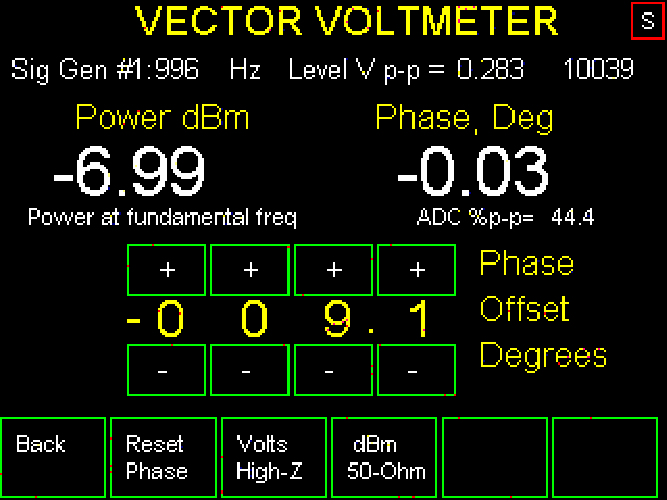
\includegraphics[scale=0.75]{./images/AVNA_018.pdf}
\caption{Vector Voltmeter with display set to power into 50-Ohms, expressed in dBm.}
\label{AVNA_018-label}
\end{center}
\end{figure}
%

One last note, if you are using an external signal source for VVM, and the measurements fails showing only microvolts, it is most likely that SG \#1 is not within a few Hz of the frequency of the input signal.  If the external source is not sufficiently stable, this may not be an appropriate method of measurement.  A broadband RMS voltmeter could be implemented, but that is for the future.

\subsection{Discussion}
\label{subsect:VVMDiscus}
The operation of the VVM is worthy of a few words. As a test instrument, it is closely related to the transmission measurements part of the Vector Network Analyzer AVNA). Much software is shared between the two instruments. The AVNA determines the relative gain or loss, amplitude and phase, through the transmission path. The VVM is calibrated so that the magnitude of the incoming signal is measured, along with the phase difference between Signal Generator \#1 and the incoming signal.

\subsection{DSP Circuit} Two mixer (multiplier) outputs are the in-phase and quadrature signal levels. The square root of the sum of the squares of these two provides the magnitude of the incoming signal. The Signal Generator \#1 (SG \#1) sets the frequency of the measurement. Low pass filtering after the mixers sets the requirement that the incoming signal must be within a few Hz of the SG \#1 frequency. In many cases, it is easiest to just use the Signal Generator output on the \q{Z} terminals of the AVNA1 which is both on frequency and without time-varying phase.

If the SG \#1 signal is used as a signal source, the phase will not be shifting with time with time. For this the phase offset can be useful. This has up/down buttons to allow setting to 0.1 degree. The offset can be positive or negative. This is a convenience for zeroing the displayed phase and does not change the basic measurement.

\subsection{Input Range} The input signal needs to be within the range of the ADC. The maximum input is a little more than 0.2 Vrms or 0.6 V p-p.  Higher voltages require an external voltage divider.  The VVM can be used with a 50-Ohm input terminator; without the 50-Ohm terminator the input impedance is 1-megohm in parallel with around 25 pF.  In all cases, the VVM shows the voltage at the \q{T} input terminals.  The displayed voltage is the RMS value.  This is the same as HP used on the (now  old) 8405A VVM.   If the waveform is not sinusoidal, and there are harmonics, the displayed value is for the fundamental at the frequency of SG \#1.

The very narrow bandwidth of the VVM allows low level signals to be measured.  With SG \#1 turned off, there is a residual noise of about 10 microVolts.  To use an external source generator, the SG \# 1 must be tuned to the same frequency.  Otherwise, leakage through the CAL switch U4B in the AVNA1 causes a signal of about 55 uV with the 50 Ohm terminator or around 1.5 mV without the 50-Ohm terminator

\textbf{Single Channel Limitations - }The HP 8405 VVM has two inputs and phase-locked tuning to the reference input.  The AVNA1 only has one input channel, so the two channel feature cannot be supported.  But wait, there actually are two inputs.  If the AVNA was rewired to remove R46 to R49 and bring those leads to a switch and to a second input connector, a full 8405A style phase-locked loop could be implemented.  But, not now!

